\chapter{Literature Review}

\section{Information and Communication Technologies in Developing Countries}
It is important to take notice of what kind of development \gls{ict}'s are supposed to support.
And in this notion make conclusions and measures based on that.
Like increase a countries competitiveness in the global free market.




Common problems that concerns the \gls{is} in developing countries are:
\begin{itemize}
\item Scarce resourses
\item Little technology
\item Missing skills
\end{itemize}

\subsection{Discourses}
\label{subsec:discourses}
\begin{itemize}
\item The pace and direction is set by the advanced economies in the world, North America and Europe. \cite{ca:isdc}
\item An increasing number of studies in developing countries in Africa, Asia and Latin America.
\item Developing countries are highlighting new topics like national culture, global politics, provision of \gls{ict} resources for a community.
\item 
\end{itemize}
\begin{description}
\item[\textit{Transfer and Diffusion Discourse}]
	The Transfer and Diffusion discourse assumes that \gls{is}-innovations in developing countries are achieved by transferring technology and organizational structure from more advanced countries. Much like, "if it works here, it should work there". In order to succeed the receiving part should try to emulate what is being done in the more developed countries. Of course \gls{is} these ideas of best practice are somewhat adapted to fit their new context, but the underlying assumption is that the transferred methods result in the same outcomes.
\item[\textit{Social Embeddednes Discourse}]
	This discourse assumes that \gls{is} innovation is about creating new techno-organizational structures given a local social context. The new structures are built on the already existing structures and are a locally socially constructed course of action. The problems are seen from a local perspective and hence the solutions has to be an integrated part.
\item[\textit{Transformative Discourse}]
	The last discourse is mostly concerned with creating possibilities for improvement of life conditions. It focuses on how \gls{is} can be used to facilitate deep socio-economic change.
	The social embeddednes discourse takes the local context into consideration, but the transformative takes it one step further and includes politics, economics and social conditions. 
\end{description}

The transformative discourse raises more explicitly the strategic issues in the development struggle.

A distinctive feature of \gls{is} research in developing countries is that it puts focus on e-governments, free and open software and the development of community resources intended to overcome the digital divide.

Issues that received attention in \gls{isdc}.
\begin{itemize}
\item \gls{is}-failure
\item Outsourcing
\item The strategic role of \gls{ict}
\end{itemize}

\cite{ca:isdc}

\subsection{Success and Failure of ISDC}
\label{successandfailure}

Are there any evidence suggesting that there are more \gls{is}-failures in developing countries?




In the \gls{isdc} literature the is an anxiety about failure, and not without reason.
Compared to other settings there are additional pressures.
The need to catch up with the rest of the world, high opportunity costs and over optimistic expectations.




Categories of failure:
\begin{itemize}
\item Scalability failure because of waning political support, technological complexity, human resource capacity.
\item Sustainability failure because of starvation of \gls{is} resource, loose political commitment, poorly maintained. This could be tracked down to foreign aid-donors that neglected the development of local technological capabilities. The remedy is of course to look at \gls{is} as the socially embedded instead of transfer and diffusion. The \gls{is} project needs to be an integrated part of organizational practices, secure the required financial and knowledge based resources and political commitment in order to succeed.
\item Assimilation in dysfunctional organizational processes, meaning that an already broken system cannot be fixed with facilitating the broken system with \gls{is}.
\end{itemize}





\begin{description}
\item[Total Failure] An initiative that never is implemented or abandoned immediately after implementation.
\item[Partial Failure] An initiative where major goals are unattained or where there are significant undesirable outcomes.
\item[Success] An initiative where major goals are attained for most stakeholders and there are no significant undesirable outcomes.
\end{description}




\begin{figure}
\centering
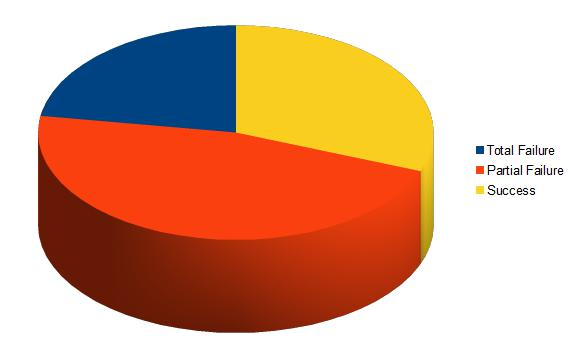
\includegraphics[width=\textwidth]{literature/img/failChart}
\caption{Diagram of Success and Failures in Industrialized Countries}
\label{fig:failchart}
\end{figure}

In industrialized countries there is an estimate of $\frac{12}{60}$ to $\frac{15}{60}$ fall into the category of total failure; something like $\frac{20}{60}$ to $\frac{36}{60}$ fall in the partial failure category; and lastly the $\frac{9}{60}$ to $\frac{28}{60}$ are successes. See figure \ref{fig:failchart}.

For practical reasons like lack of technical and human infrastructure developing countries should be performing worse than industrialized countries.
The evidence base is not that strong due to lack of literature in general, evaluation and focus on case studies, but it generally points in one direction. High rates of \gls{is}-failure.

Failure can be viewed as something positive. 
Like in a learning process, but it cannot be overlooked that continually failing keeps the under developed countries on the wrong side of the digital divide. 

Organizational change can be viewed as a process between two states.
The current system and the future.
The future system would represent the design of a \gls{is} system that are to be implemented.
And the current system as a description of how the system is.
Between these models there will need to be some change in several dimensions like processes, people, structure and technology in order to reach the a state of the future system. This design-actuality gap usually represents how much risk are involved from moving to a design. 

The actuality of the industialized countries and developing countries have in themselves gaps.
The design-actuality gap might not be the same for the solutions used in industrialized countries and developing countries. 

\cite{rh:isdc}
\cite{ca:isdc}


\section{Outsourcing}
A number of developing countries have nurtured software and \gls{ict} services industries able to compete in the global market, India being the most successful. 
Factors that account for success in the global market include technology and project management skills, copyright legislation and government industrial policy. By making an effort to outsource, there may be also be an increase to services offered to the domestic organizations. This in turn will have an impact on the overall developments of the country or region. It is hard to imagine that there are little technological use in a place that are among the top exporters of software. The spill over effect may results in local organizations running better, and this way offering better possibilities in the other fields as well.

\cite{ca:isdc}






\section{Digital Divide}

\section{E-Health}
E-health is defined as:
\begin{quotation}
Use of information and communications technologies in support of health and health-related fields, including health-care services, health surveillance, health literature, and health education, knowledge and research.
\end{quotation}

E-health has many areas of application. Studies have shown that in by using electronic health records it is possible to improve staff productivity, reducing patient wait times, increase staff satisfaction and providing higher quality of data to relevant personnel. Laboratory information managements systems have decreased the time for communicating results and improved the productivity of the laboratory. Pharmacy information systems reduces time to order medications and provides easy access to past information. This is useful for forecasting medication requirements in order to get it at a lower price. Particularly relevant for drug resistant \gls{tb} medications. Also reducing the number of errors. Fingerprint scanners reduced the time to locate records with 74\% and barcode scanners reduced the time by 97\%. The time to track patients lost to follow-up could with patient tracker systems be reduced by 20--50\%. And patient reminder systems can increase attendance with up to 21\%. A cost analysis of data collection systems show that it is possible to save 91\% over a paper based system. 

These findings clearly argue for the implementation and commitment of e-health in developing countries. 

Challenges include:
\begin{itemize}
\item physical environment
\item power
\item networking
\item availabillity of technical staff
\end{itemize}

\cite{ehealth:blaya}

\section{Transition Strategy}
With a transition I talk about taking the system as it is and change it to something new. 
It's the process from old to new. The process of transforming systems or system migration if you will.

Making a transition involves a switch from the old system to the new. There
is the source system, also referred to as the legacy system and the target
system. At one end of the specter we have the Big Bang strategy, were we
taken on an revolutionary approach. A complete new system is developed,
supporting all the required functionality. Then one decideds a time when all
of those involved switches to the new system. This way usually has a high
risk of failure. On the other end of the spectrum we have the evolutionary
approach. Gradually one introduces new functionality, or the same with a
new system, then after the legacy system is not used anymore, one turns off
the switch.

\subsection{Planning and Conducting a Transition Strategy}
There are some predefined methods for conducting a system migration which
also could be used in a transition strategy plan. Remembering that one
moves from a source system into a target system. As mentioned, solutions to
transition problems could be characterized by how revolutionary it is. The
most revolutionary would be redevelopment, followed by migration, maintenance and finally wrapping. One would choose the most appropriate strategy based on the level of risk. 
Like wrapping, one takes almost no risk, since it requires no real change to the system, but instead provides an updated interface for the source system. Although this way is low risk, this could complicate things later on. Making use of wrapping not only slows down the system,
but also makes maintenance more complicated. The most appropriate use of
wrapping is when one wants to make a new Graphical User Interface (GUI).
Like when moving from a text based front-end to a graphical based front-end.
With redevelopment on one end and wrapping on the other, in the middle we
have system migration. This technique allows for a smoother approach while
being able to have control.

\subsection{Migration}
When redevelopment is to risky and wrapping is unsuitable, migration usu-
ally is the best way to go. This allows for both systems to co-exist while
making the transition from one to the other. Migration usually involves
moving an existing system to a new platform. Before making the transition
one has to decide on some basics. Like how one would like to migrate to the
new system. Much of the time is spent on testing the target system. There-
fore it is good practice to not introduce new functionality while migrating to
a new platform. It also makes the testing easier since one could compare with
the old system for output results. New functionality should be introduced
afters the old ones are supported.

\subsubsection{The Cutover}
The cutover is the last step in the migration process. 
Here are three main approaches.

\begin{description}
\item[The cut and run] This is the most revolutionary way of migrating. It is
much like redevelopment and seldom used alone. Once the target sys-
tem is ready on turns of the source system and enable a new feature
rich system.

\item[Phased interoperability] In this strategy incremental steps towards the
target system is used. Replacing functionality over time and slowly
moving towards target system until all functionality is replaced. The
last part of the cutover would be cut and run to some degree.

\item[Parallell operations] In this strategy both systems are running at the same
time. Both source and target system is operational. The target system
is continually tested and only when it's fully trusted, the source system
is disabled.
\end{description}

The cut and run is very simple, but usaually involves high risk. Parallell
operations usually become quite complex, but are fairly safe. Phased interoperability is somewhere in the middle.

\cite{leg:jdbj}


\section{Groupware}
Groupware development is found among the developers.
When the purchasers buy visible and expensive systems organizational change is likely.
Upper managements is thus likely to commit to helping the system succeed.
Social and political factors that affect the introduction of a system.
\begin{itemize}
\item job redesign 
\item job creation
\item providing training
\item restructuring to work around individuals who will not use the system
\item positive leadership
\end{itemize}

Management is less committed to the less expensive applications or features.
An organization will not restructure itself for each new application the way it does around a major new system. Therefore these systems must adapt to the organization and be fitted into existing work patterns and appealing to everyone who must support it. 

\section{Information systems in the learning economy}
\label{infolearnec}
Research in developed countries has shown that learning is a critical factor for economic success.
This is not just critical for firms and industries, but also for regions and countries.
This makes learning a crucial factor for developing countries. 
Learning, being an interactive socially embedded process, are facilitated through the institutional setup or the national innovation system. It's efficiency very much depends on the circumstances.
By making the environment facilitate learning one has the opportunity to increase learning, and in turn, better the economy and technology, making living conditions better. 
Through \gls{ict}, knowledge can be spread from one individual to another. 
By actively making \gls{ict}'s available we also are making knowledge available and facilitating the learning process. 
So with efforts focused on \gls{ict}'s, developing countries are able to learn faster by having greater access to knowledge and as a result having a better economy.
This would actually just take the developing countries to a level already reached by the developing countries. So in order to really have an impact, they would need to have an advantage. 
Japan and \gls{usa} have two very successful, but different approaches to learning. 
The one from \gls{usa} has a focus on explicit knowledge. Here the focus is on reducing tacit knowledge into information with clearly defined processes and facts. A good example at this would be a step-by-step guide in order to learn something new. 
On the other hand Japan has more focus on making tacit knowledge. This is the knowledge that is almost subconscious. You don't necessarily know it as a set of instructions. This learning strategy are often built on the master-apprentice scheme focusing on co-operation, social cohesion and long-term social relationships. 
By acknowledging that there are two types of strategies, there must be a third that combines the best from both. 
Now, since success in the global economy are based on learning there are an opportunity here for the developing countries to not only advance to the level of the developed, but also have an advantage. 

\cite{gedi:erik}

\section{Outsourcing}
Offshoring has it's spring from:

\begin{itemize}
\item globalization of trade in services
\item Software commoditization
\item Wage differentials
\item Business friendly climate 
\item Growth of offshore labor pool
\item Drop in telecom costs
\end{itemize}

China graduates four times more engineers than the \gls{usa} pr. year. 
Before there were a differance in the quality of the engineering program, but the gap has narrowed. 
The talent was always there, but before those with talent would emigrate to industrialized countries. 
With globalization of trade in services we can tap into their services from anywhere. 
With low telecom prizes, low wages and software commoditization industrialized countries are able to offshore their software activities more or less. 

The wage factor are the most dominant factor for off-shoring.
The global software work phenomenon is not the first of it's kind, but it differs in that it delivers a service rather than a specific product. 
It is well known that manufactoring and production are often moved to other low-wage countries.
Parts of software development has now become such a commodity that firms from industrialized countries are able to outsource these tasks and keep the more high-level activity for themselves. 

A useful way of understanding this context is via Vernon's \textit{international product cycle}.
\begin{description}
\item[\textit{Stage 1:}]\hfill
A new product begin with highly skilled entrepreneural activities, typically in industrialized nations.
\item[\textit{Stage 2:}]\hfill
Production begin to shift offshore via investments in low-wage nations.
\item[\textit{Stage 3:}]\hfill
As the product standardizes, it is mass produced with cheap, low-skilled labor.
\end{description}


Software has areas in all three stages. The high-level activities stay in stage 1 while being prepared as routine tasks of best practice, then moved towards stage 3 through stage 2.

Global Software Work opens up a market that are very different from others.
The developing countries are here able compete under very different circumstances.
Were the developed countries has to deal with high salaries the developing countries can benefit from having lower salaries and compete on cost. This makes the market highly dependent on the knowledge competencies. As discussed in section \ref{infolearnec} a countries ability to learn has a great impact for developing the economy. Access to knowledge intuitively has a way of speeding up the learning process. And the most efficient way of getting to knowledge is through \gls{ict}'s. 
Having the opportunity to compete on knowledge competencies can pace the way for developing countries. By focusing on learning the developing countries of the world are able to enter the market of \gls{ict}'s with an advantage. Policy makers in charge of economic growth and infrastructure should therefore recognize this and facilitate both the learning process and the exportation of services. 
By focusing on this area of expertise development in other areas of industry are likely.
Having a highly developed \gls{ict} infrastructure is likely to have spillover effects on the domestic services and production. Making opportunities for even new innovations. 
History has shown that there is a link between fortunes of the developed countries and the developing. Rapid upgrades in \gls{ict}'s have reduced the costs and increased the scope of operations all over the world. 


\cite{sbs:gio}
\cite{offit:paan}